\section{Analysis}\label{sec:Analysis}
Since the early 1960s, the Calcium Fraunhaufer lines have been used as
chromospheric activity tracers \citep{Wil63}. Ca II H\&K lines are observed as
a combination of a broad absorption feature originating in the upper
photosphere along with a narrow emission feature from non-thermal heating of
the upper chromosphere \citep{Catalano1983}. Specifically, the ratio between
emission in the Ca II H\&K lines and flux contributed from the photosphere is
used to define an activity metric known as the S-index \citep{Wil68}.   The
S-index increases with increasing magnetic activity. The S-index is defined as 

\begin{equation}\label{eqn:SIndex}
    S = \alpha \frac{f_{H} + f_{K}}{f_{V} + f_{R}}    
\end{equation}

\noindent where $f_{H}$  and $f_{K}$ are the integrated flux over triangular
passbands with a full width at half maximum of $1.09\text{ \AA}$ centered at
$3968.47\text{ \AA}$ and $3933.66\text{ \AA}$, respectively. The values of
$f_{V}$ and $f_{R}$ are integrated, top hat, broadband regions. They
approximate the continuum (Figure \ref{fig:SindexBandpass}) and are centered at
3901 \AA \ and 4001 \AA \ respectively, with widths of 20 \AA \ each. Finally,
$\alpha$ is a scaling factor with $\alpha = 2.4$.

\begin{figure*}[ht!]
    \centering
    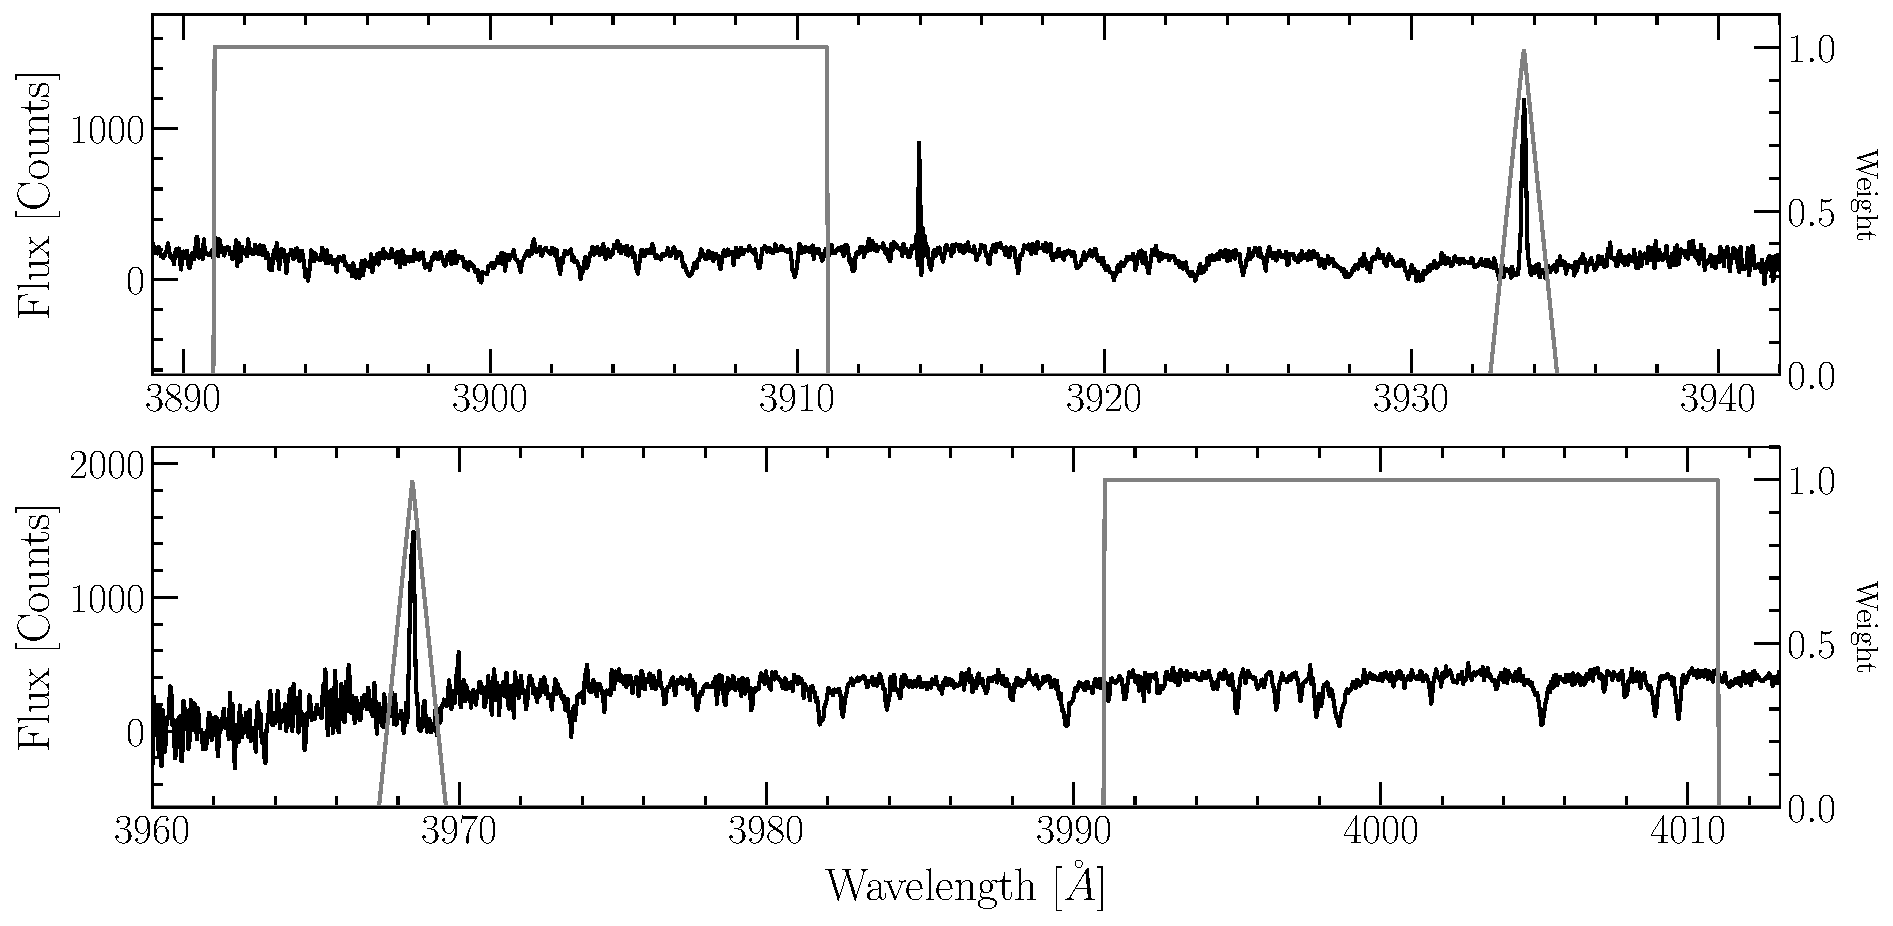
\includegraphics[width=0.9\textwidth]{figures/magActivity/SIndexBandpass.pdf}
	\caption{Spectrum of 2MASS J06105288-4324178 overplotted with the S index
	bandpasses. (top) V band and Ca II K emission line. (bottom) Ca II H
	emission line and R band. Note that the rectangular and triangular
	regions denote both the wavelength range of the band and the relative
	weight assigned to each wavelength in the band while integrating. }
    \label{fig:SindexBandpass}
\end{figure*}

Following the procedure outlined in \citet{Lov11} we use the mean flux per
wavelength interval, $\tilde{f_{i}}$, as opposed to the integrated flux over
each passband when computing the S-index. This means that for each passband,
$i$, with a blue most wavelength $\lambda_{b,i}$ and a red most wavelength
$\lambda_{r,i}$, $\tilde{f}_{i}$ is the summation of the product of flux ($f$)
and weight ($w_{i})$ over the passband.

\begin{equation}\label{eqn:meanFlux}
    \tilde{f}_{i} = \frac{\sum_{l = \lambda_{b,i}}^{\lambda_{r,i}}f(l)w_{i}(l)}{\lambda_{r,i}-\lambda_{b,i}}    
\end{equation}
\noindent where $w_{i}$ represents the triangular passband for $f_{H}$ \& $f_{K}$ and the tophat for $f_{V}$ \& $f_{R}$.

Additionally, the spectrograph used at Mount Wilson during the development of
the S-index exposed the H \& K lines for eight times longer than the continuum
of the spectra. Therefore, for a modern instrument that exposes the entire
sensor simultaneously, there will be 8 times less flux in the Ca II H\&K
passbands than the continuum passbands than for historical observations. This
additional flux is accounted for by defining a new constant $\alpha_{H}$,
defined as:

\begin{equation}
    \alpha_{H} = 8\alpha\left(\frac{1.09\text{ \AA}}{20\text{ \AA}}\right)
\end{equation}
Therefore, S-indices are calculated here not based on the historical definition
given in Equation \ref{eqn:SIndex}; rather, the slightly modified version:

\begin{equation}\label{eqn:finalSIndex}
    S = \alpha_{H}\frac{\tilde{f}_{H} + \tilde{f}_{K}}{\tilde{f}_{V} + \tilde{f}_{R}}
\end{equation}

The S-index may be used to make meaningful comparisons between stars of similar
spectral class; however, it does not account for variations in photospheric
flux and is therefore inadequate for making comparisons between stars of
different spectral classes. The $R'_{HK}$ index \citep{Middelkoop1982} is a
transformation of the S-index intended to remove the contribution of the
photosphere. 

$R'_{HK}$ introduces a bolometric correction factor, $C_{cf}$, developed by
\citet{Middelkoop1982} and later improved upon by \citet{Rutten1984}.
Calibrations of $C_{cf}$ have focused on FGK-type stars using broad band color
indices, predominately B-V. However, these FGK-type solutions do not extend to
later type stars easily as many mid-late M-dwarfs lack B-V photometry.
Consequently, $C_{cf}$ based on B-V colors were never calibrated for M-dwarfs
as many M-dwarfs lack B and V photometry. \citet{SuarezMascareno2016} provided
the first $C_{cf}$ calibrations for M-dwarfs using the more appropriate color
index of $V-K$. The calibration was later extended by \citet{Def17}, which we
adopt here. 

Generally $R'_{HK}$ is defined as

\begin{equation}\label{eqn:RpHKDef}
    R'_{HK} = K\sigma^{-1}10^{-14}C_{cf}(S-S_{phot})
\end{equation}
where K is a factor to scale surface fluxes of arbitrary units into physical
units; the current best value for K is taken from \citet{Hal07},
$K=1.07\times10^{6}\text{erg cm$^{-2}$ s$^{-1}$}$. $S_{phot}$ is the
photospheric contribution to the S-index; in the spectra this manifests as the
broad absorption feature wherein the narrow Ca II H\&K emission resides.
$\sigma$ is the Stephan-Boltzmann constant. If we define 

\begin{equation}
    R_{phot}\equiv K\sigma^{-1}10^{-14}C_{cf}S_{phot}
\end{equation}
then we may write $R'_{HK}$ as 

\begin{equation}\label{eqn:RpHKFinal}
    R'_{HK} = K\sigma^{-1}10^{-14}C_{cf}S - R_{phot}.
\end{equation}

We use the color calibrated coefficients for $\log_{10}(C_{cf})$ and
$\log_{10}(R_{phot})$ presented in Table 1 of \citet{Def17}.

We estimate the uncertainty of $R'_{HK}$ as the standard deviation of a
distribution of $R'_{HK}$ measurements from 5000 Monte Carlo tests. For each
science target we offset the flux value at each wavelength bin by an amount
sampled from a normal distribution. The standard deviation of this normal
distribution is equal to the estimated error at each wavelength bin. These
errors are calculated at reduction time by the pipeline. \textbf{The R$'_{HK}$
uncertainty varies drastically with signal-to-noise; targets with
signal-to-noise ratios $\sim 5$ have typical uncertainties of a few percent
whereas targets with signal-to-noise ratios $\sim 100$ have typical
uncertainties of a few tenth of a percent.}

\subsection{Rotation and Rossby Number}
The goal of this work is to constrain the rotation activity relation;
therefore, in addition to the measured $R'_{HK}$ value, we also need the
rotation of the star. As mentioned, one of the selection criteria for targets
was that their rotation periods were already measured; however, ultimately
\textbf{6} of the 53 targets with acceptable S/N did not have well constrained
rotational periods. We therefore only use the remaining 47 targets to fit the
rotation-activity relation. 

% In order to make the most meaningful comparison possible we transform rotation
% period into Rossby Number . This transformation was done using the convective
% overturn timescale, $\tau_{c}$, such that the Rossby Number, $Ro =
% \frac{P_{rot}}{\tau_{c}}$ . To first order $\tau_{c}$ can be approximated as
% $70$ days for fully-convective M-dwarfs \citep{Pizzolato2000}. However,
% \citet{Wri18} Equation (5) presents an empirically calibrated expression for
% $\tau_{c}$. This calibration is derived by fitting the convective overturn
% timescale as a function of color index, in order to minimize the horizontal
% offset between stars of different mass in the rotation-activity relationship.
% The calibration from \citet{Wri18} that we use to find convective overturn
% timescales and subsequently Rossby numbers is:

In order to make the most meaningful comparison possible we transform rotation
period into Rossby Number . This transformation was done using the convective
overturn timescale, $\tau_{c}$, such that the Rossby Number, $Ro =
P_{rot}/\tau_{c}$ . To first order $\tau_{c}$ can be approximated as $70$ days
for fully-convective M-dwarfs \citep{Pizzolato2000}. However, \citet{Wri18}
Equation (5) presents an empirically calibrated expression for $\tau_{c}$. This
calibration is derived by fitting the convective overturn timescale as a
function of color index, in order to minimize the horizontal offset between
stars of different mass in the rotation-activity relationship.  The calibration
from \citet{Wri18} that we use to find convective overturn timescales and
subsequently Rossby numbers is:

\begin{equation}\label{eqn:convectiveOverturn}
    \log_{10}(\tau_{c}) = (0.64\pm0.12)+(0.25\pm0.08)(V-K)
\end{equation}
We adopt symmetric errors for the parameters of Equation
\ref{eqn:convectiveOverturn} equal to the larger of the two anti-symmetric
errors presented in \citet{Wri18} Equation 5. 
